\documentclass[pdflatex,sn-mathphys-num]{sn-jnl}

\usepackage{graphicx}
\usepackage{multirow}
\usepackage{amsmath,amssymb,amsfonts}
\usepackage{amsthm}
\usepackage{mathrsfs}
\usepackage[title]{appendix}
\usepackage{xcolor}
\usepackage{textcomp}
\usepackage{manyfoot}
\usepackage{booktabs}
\usepackage{algorithm}
\usepackage{algorithmicx}
\usepackage{algpseudocode}
\usepackage{listings}

\raggedbottom

\begin{document}

\title[Evaluación de Modelo Base: Regresión Logística]{Clasificación de la Aptitud Solar Fotovoltaica a Partir de Variables Geoespaciales y Climáticas: Evaluación de un Modelo Base de Regresión Logística (Segunda Entrega)}

\author*[1]{\fnm{Jesús David} \sur{Arévalo Montilla}}\email{jdarevalo@uninorte.edu.co}

\author[1]{\fnm{Enmanuel David} \sur{Diaz Molinares}}\email{denmanuel@uninorte.edu.co}

\author[1]{\fnm{Alex David} \sur{Teran Meza}}\email{talex@uninorte.edu.co}

\affil*[1]{\orgdiv{Departamento de Matemáticas y Ciencia de Datos, Programa de Ciencia de Datos}, \orgname{Universidad del Norte}, \orgaddress{\city{Barranquilla}, \country{Colombia}}}

\abstract{Esta segunda entrega evalúa un único modelo de clasificación (Regresión Logística multinomial) sobre el problema de aptitud solar planteado en la primera entrega, con el fin de establecer un margen de mejora concreto que las siguientes entregas buscarán cerrar. Se usan las 17 variables predictoras definidas en el Análisis Exploratorio de Datos (13 numéricas, con imputación por mediana en \texttt{area}, y 4 categóricas codificadas con one-hot) para predecir \texttt{solar\_aptittude\_class} (Baja, Media, Alta) sobre las 58{,}978 plantas del \textit{Global Solar Power Plants Dataset}. El modelo base, sin ajuste alguno, alcanza una exactitud de 0.787 en el conjunto de prueba pero un recall de apenas 0.57 para la clase minoritaria (Baja, 3.21\% del dataset). Incorporando \texttt{class\_weight='balanced'} y optimizando el hiperparámetro de regularización $C$ mediante \texttt{GridSearchCV} con validación cruzada estratificada de 5 particiones, el recall de Baja sube a 0.97, a costa de una caída moderada de exactitud (a 0.753) y de F1 macro (de 0.65 a 0.62). El ROC AUC macro (0.886) se mantiene idéntico entre ambas versiones, lo que confirma que la capacidad discriminativa real del modelo no cambia: lo que cambia es el umbral de decisión que la ponderación de clases desplaza hacia la clase minoritaria. Estos resultados fijan la referencia de desempeño que los modelos evaluados en la siguiente entrega deberán superar.}

\keywords{Regresión logística multinomial, Clasificación multiclase desbalanceada, Aptitud solar fotovoltaica, Ponderación de clases, ROC AUC macro}

\maketitle

\section{Introducción}\label{sec:intro}

La primera entrega de este proyecto estableció, mediante un Análisis Exploratorio de Datos exhaustivo sobre el \textit{Global Solar Power Plants Dataset} \cite{bib1}, que la clasificación de la aptitud solar de un sitio (\texttt{solar\_aptittude\_class}: Baja, Media, Alta) es un problema de clasificación multiclase fuertemente desbalanceado (75.10\% Alta, 21.69\% Media, 3.21\% Baja), con 17 variables predictoras válidas (13 numéricas y 4 categóricas) que describen terreno y clima sin incurrir en fuga de datos.

Antes de comparar modelos más complejos entre sí, es necesario cuantificar qué tan lejos está un modelo lineal simple de resolver el problema, y en qué dimensión falla exactamente. La Regresión Logística multinomial \cite{bib2} es la elección natural para este propósito: es interpretable, computacionalmente económica, y su comportamiento bajo desbalance de clases está bien documentado en la literatura \cite{bib3}, lo que permite atribuir con claridad cualquier falla observada al desbalance de clases y no a la complejidad del modelo.

Esta entrega tiene un objetivo distinto al de una comparación de modelos: identificar el margen de mejora concreto que separa a un modelo base de un desempeño aceptable en la clase minoritaria, y verificar si ese margen puede cerrarse parcialmente con ajustes propios de la regresión logística (ponderación de clases, regularización), antes de introducir modelos de mayor capacidad en la siguiente entrega. En este trabajo entrenamos un modelo base de Regresión Logística y una versión con \texttt{class\_weight='balanced'} y regularización optimizada por búsqueda en grilla, y mostramos que, aunque el ajuste mejora sustancialmente el recall de la clase minoritaria, persiste un margen de mejora relevante en F1 macro que motiva la comparación con modelos no lineales en las próximas entregas.

\section{Metodología}\label{sec:metodologia}

\subsection{Datos y variables predictoras}\label{subsec:datos}

Se utiliza el mismo conjunto de datos y las mismas 17 variables predictoras validadas en la primera entrega: 13 numéricas (\texttt{longitude}, \texttt{latitude}, \texttt{elevation}, \texttt{area}, \texttt{slope}, \texttt{curvature}, \texttt{aspect}, \texttt{dist\_to\_road}, \texttt{ambient\_temperature}, \texttt{ghi}, \texttt{humidity}, \texttt{wind\_speed}, \texttt{wind\_direction}) y 4 categóricas (\texttt{slope\_type}, \texttt{curvature\_type}, \texttt{aspect\_type}, \texttt{dt\_wind}). Se excluyen \texttt{solar\_aptitude}, \texttt{solar\_aptitude\_rounded}, \texttt{capacity}, \texttt{optimal\_tilt}, \texttt{pv\_potential} y \texttt{operational\_status} por fuga de datos o por ser posteriores a la decisión de inversión, y los identificadores \texttt{OBJECTID}, \texttt{code} y \texttt{plant\_name} por no tener valor predictivo.

Los datos se dividen en 80\% entrenamiento y 20\% prueba mediante partición estratificada (semilla aleatoria 42). El preprocesamiento se aplica dentro de un \texttt{ColumnTransformer} ajustado únicamente sobre el conjunto de entrenamiento: las variables numéricas se imputan con la mediana (necesario solo para \texttt{area}, con 27.69\% de nulos) y se estandarizan; las 4 variables categóricas se codifican con \textit{one-hot encoding}. El vector de entrada final tiene 39 columnas (13 numéricas más 26 columnas binarias de las categóricas).

\subsection{Modelo evaluado}\label{subsec:modelo}

Se evalúa una Regresión Logística multinomial \cite{bib2}, que modela la probabilidad de cada clase $k \in \{\text{Baja}, \text{Media}, \text{Alta}\}$ mediante la función softmax sobre combinaciones lineales de las variables de entrada,

\begin{equation}
P(y = k \mid x) = \frac{\exp(w_k^\top x + b_k)}{\sum_{k'} \exp(w_{k'}^\top x + b_{k'})},
\label{eq:softmax}
\end{equation}

\noindent y se entrena minimizando la log-verosimilitud negativa regularizada con norma $L_2$,

\begin{equation}
\min_{\{w_k, b_k\}} \; \frac{1}{C}\sum_{k} \lVert w_k \rVert_2^2 \; - \sum_{i=1}^{n} \log P(y_i \mid x_i),
\label{eq:logloss}
\end{equation}

\noindent donde $C$ controla el inverso de la fuerza de regularización. Se entrenan dos versiones: un modelo base sin ajuste de hiperparámetros ni ponderación de clases, y una versión con \texttt{class\_weight='balanced'} (que pondera cada término de la log-verosimilitud por el inverso de la frecuencia de su clase, siguiendo el tratamiento estándar de regresión logística bajo eventos raros \cite{bib3}), con $C$ optimizado por búsqueda en grilla.

\subsection{Configuración experimental}\label{subsec:config}

Se usan como métricas la exactitud (accuracy), precisión, recall y F1-score por clase, F1 macro, y ROC AUC macro en esquema uno-contra-el-resto, apropiadas para un problema multiclase desbalanceado donde la exactitud global puede ser engañosa. El hiperparámetro $C \in \{0.01, 0.1, 1, 10, 100\}$ se ajustó mediante \texttt{GridSearchCV} optimizando F1 macro, con \texttt{StratifiedKFold} de 5 particiones sobre el conjunto de entrenamiento. Todo el pipeline se implementó en Python 3.14 con scikit-learn \cite{bib4}; el entrenamiento y la evaluación se ejecutaron en CPU, sin requerimientos de hardware especializado dado el tamaño del modelo.

\section{Resultados}\label{sec:resultados}

La Tabla~\ref{tab:resultados} resume el desempeño del modelo base y del modelo ajustado sobre el conjunto de prueba. El modelo base ya supera con margen amplio al conjunto de features usado en una iteración previa de este mismo modelo (que producía un recall de Baja cercano a 0, al incluir por error \texttt{optimal\_tilt} en vez de \texttt{slope}/\texttt{aspect}/\texttt{curvature}); con las variables correctas, el modelo base identifica más de la mitad de las plantas Baja sin ningún ajuste. La búsqueda en grilla seleccionó $C=10$, con un F1 macro promedio de 0.638 en validación cruzada.

\begin{table}[h]
\caption{Desempeño del modelo base y del modelo con ponderación de clases y $C$ optimizado, sobre el conjunto de prueba (20\% de los datos, partición estratificada).}\label{tab:resultados}
\begin{tabular}{@{}lccccc@{}}
\toprule
Modelo & Exact. train & Exact. test & Recall (Baja) & F1 macro & ROC AUC macro \\
\midrule
Base (sin ajustar) & 0.788 & 0.787 & 0.57 & 0.65 & 0.886 \\
\texttt{class\_weight='balanced'}, $C=10$ & 0.760 & 0.753 & \textbf{0.97} & 0.62 & 0.886 \\
\botrule
\end{tabular}
\end{table}

Ponderar las clases y ajustar $C$ eleva el recall de Baja de 0.57 a 0.97, prácticamente identificando la totalidad de las plantas de baja aptitud, a cambio de una caída moderada de exactitud (3.4 puntos porcentuales) y de F1 macro (de 0.65 a 0.62), consecuencia de que el modelo ajustado sacrifica precisión en Baja (0.28) y en Alta para ganar recall. El ROC AUC macro, que no depende del umbral de decisión, es idéntico en ambas versiones (0.886, Figura~\ref{fig:confusion}), lo que indica que la capacidad discriminativa del modelo no cambió: la ponderación de clases desplazó el umbral de decisión hacia la clase minoritaria, sin alterar el ordenamiento de probabilidades que el modelo aprende.

\begin{figure}[h]
\centering
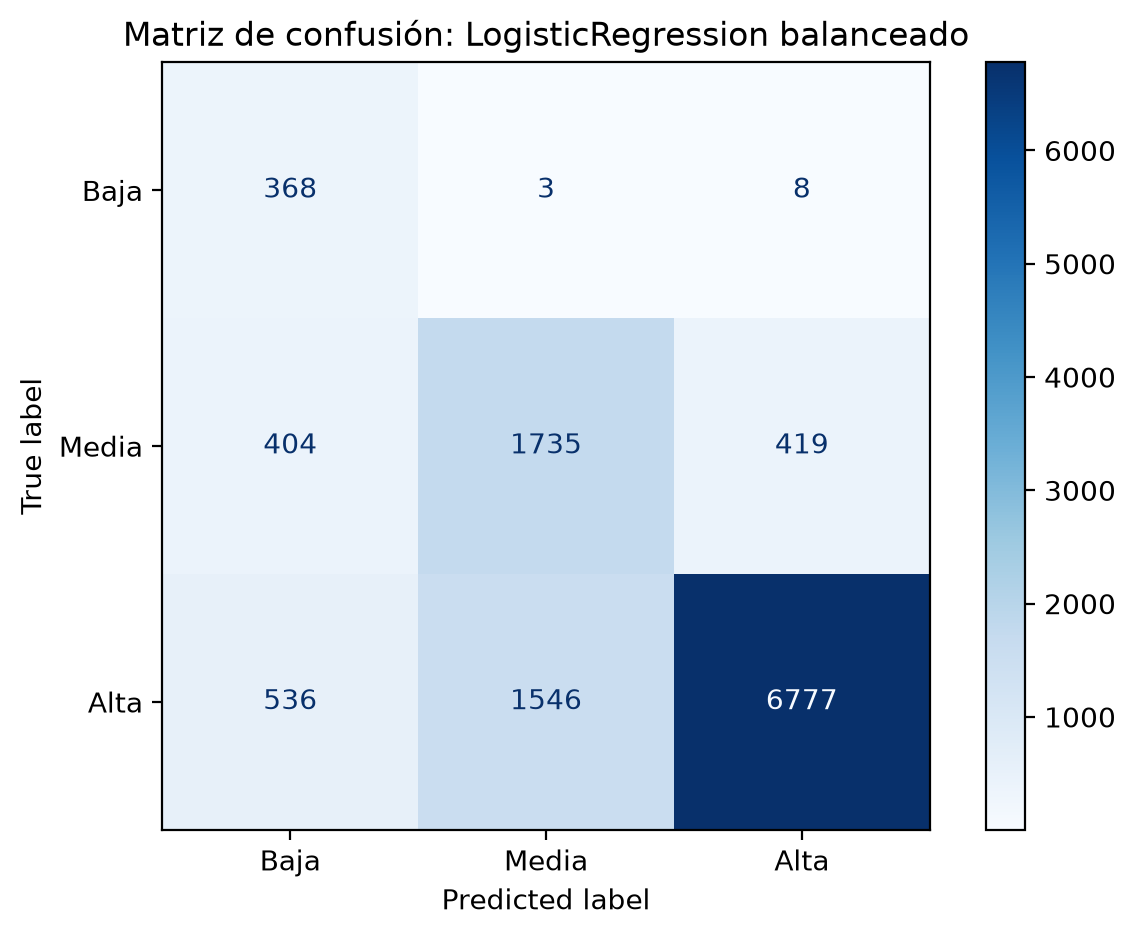
\includegraphics[width=0.55\textwidth]{fig_matriz_confusion.png}
\caption{Matriz de confusión del modelo con \texttt{class\_weight='balanced'} y $C=10$ sobre el conjunto de prueba. La clase Baja se identifica casi en su totalidad (368 de 379), a costa de que una fracción considerable de Alta y Media se reclasifique como Baja o Media.}
\label{fig:confusion}
\end{figure}

La Figura~\ref{fig:confusion} muestra que la ganancia en recall de Baja se paga principalmente con una redistribución de la clase Alta: 536 de 8{,}859 plantas Alta se reclasifican como Baja y 1{,}546 como Media. Dado que en esta entrega se evalúa un único modelo, no se realiza una prueba de significancia estadística entre versiones; esta comparación formal frente a otros modelos se reserva para la siguiente entrega, una vez incorporados los modelos adicionales del curso.

\section{Conclusiones}\label{sec:conclusiones}

El modelo base de Regresión Logística, entrenado sobre las 17 variables validadas en la primera entrega, deja un margen de mejora claro y cuantificable: su exactitud de 0.787 esconde un recall de apenas 0.57 para la clase Baja, la que más importa identificar correctamente desde una perspectiva de decisión de inversión. Ajustar la ponderación de clases y el hiperparámetro de regularización cierra buena parte de ese margen en términos de recall (hasta 0.97), pero no en F1 macro, que de hecho baja levemente (de 0.65 a 0.62); esto evidencia que un ajuste puramente basado en el umbral de decisión de un modelo lineal no es suficiente para resolver el desbalance sin sacrificar otras clases.

Como limitación, este modelo asume fronteras de decisión lineales entre clases y no captura interacciones entre variables de terreno y clima que el Análisis Exploratorio de Datos sugirió relevantes (por ejemplo, la fuerte asociación entre \texttt{longitude} y la clase de aptitud, probablemente ligada a la composición geográfica del dataset más que a una relación física directa). El margen de mejora identificado aquí, en particular el F1 macro de 0.62 a 0.65 según la versión, es la referencia que los modelos adicionales del curso (árboles, ensambles y modelos no lineales) deberán superar en la siguiente entrega, idealmente sin el costo en exactitud observado al balancear este modelo lineal.

\section*{Referencias bibliográficas}

\begin{thebibliography}{99}

\bibitem{bib1} Mantilla-Guerra, A., Mejia-Escobar, C., Azorin-Lopez, J., Garcia-Rodriguez, J., Tarco, B.F., Santamaria, K.: Global Dataset of Solar Power Plants: Multidimensional Integration and Analysis. arXiv:2603.20601 (2026)

\bibitem{bib2} James, G., Witten, D., Hastie, T., Tibshirani, R.: An Introduction to Statistical Learning, 2nd edn. Springer, New York (2021)

\bibitem{bib3} King, G., Zeng, L.: Logistic Regression in Rare Events Data. Political Analysis \textbf{9}(2), 137--163 (2001)

\bibitem{bib4} Pedregosa, F., Varoquaux, G., Gramfort, A., Michel, V., Thirion, B., Grisel, O., Blondel, M., Prettenhofer, P., Weiss, R., Dubourg, V., Vanderplas, J., Passos, A., Cournapeau, D., Brucher, M., Perrot, M., Duchesnay, E.: Scikit-learn: Machine Learning in Python. Journal of Machine Learning Research \textbf{12}, 2825--2830 (2011)

\end{thebibliography}

\end{document}
